\documentclass{article}

\usepackage{graphicx,float}

\title{title}
\author{Author}
\date{date}

\begin{document}
\maketitle
\bigskip
\begin{abstract} The identification and removal of the seasonal component is one of the main issues in time series analysis, and it is key operation performed by national statistical agencies such as Statistics Netherlands. Several procedures exist for this goal, available in a wide range of software. The most often applied techniques are based on the use of filters.  A linear filter is proposed in this paper, which can be incorporated in existing frameworks and packages for the treatment of time series, and which identifies seasonal influences in one step, with no iteration required. The aim of the study is to evaluate the efficacy of this proposed filter. In particular, the filtered series is used as the input of a seasonal adjustment procedure, performed by JDemetra+. This latter is a software for time series seasonal adjustment recommended by the European Statistical System (ESS) and European System of Central Bank (ESCB). It incorporates two methods: X-13-ARIMA, an enhanced X-11 seasonal adjustment procedure (see Dagum, 1980), developed by the U.S. Census Bureau, and TRAMO/SEATS (see Gomez \& Maravall, 1997, and Maravall \& Sanchez, 2000), proposed by the Bank of Spain. The performance of the proposed filter is analyzed on a real time series; most of the abserved diagnostics focus on the spectral analysis.
\end{abstract}
\bigskip
\textbf{1 Introduction} A key concept in time series analysis is the decomposition of a given time series into a trend component, a seasonal component and noise. Seasonality consists in movements repeated throughout the year, with similar intensity in the same period. It means that they are expected to be predictable. Seasonal movements are often large enough such that they can mask other characteristics of the data that are of interest to analysts of current trends. Removal of the seasonal component allows to produce series whose movement are easier to evaluate over time. Indeed, seasonal movements can arise with different timing and amplitude for different time series, making hard their comparison in trend-cycle terms. In this manner, it is also easier to achieve better forecasts.\\

\begin{figure}[H]
  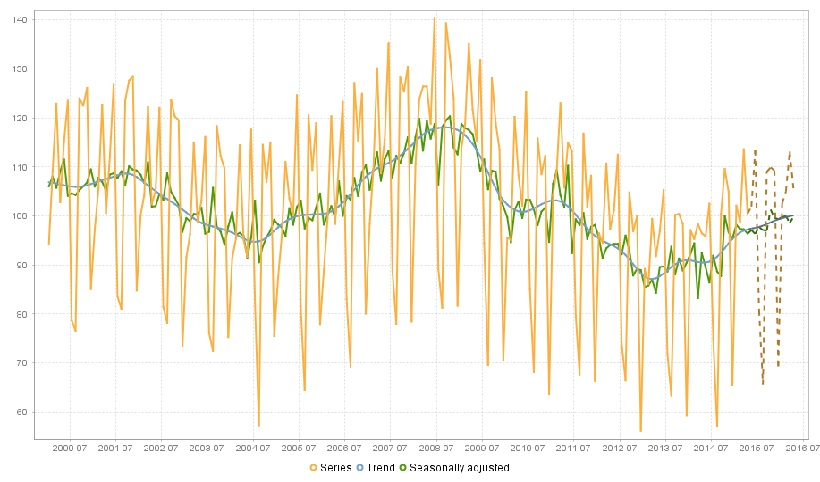
\includegraphics[width=\linewidth]{../images/capitolo1/intro.jpg}
  {\textbf{\scriptsize Figure 1: A decomposition of the Netherlands volume index of production time series in trend and seasonally adjusted series performed by JDemetra+.}}
\end{figure}

Figure 1 shows a decomposition of a time series obtained through a JDemetra+ seasonal adjustment procedure. A common method for obtaining the trend is to use linear filters on given seasonally adjusted series, and in the simplest case moving averages are considered. It means that the filtered value at time $t$ is an average of the values in a neighbour of pre-defined length of that target point. Different seasonal adjustment procedures make use of linear filters.The most often applied filters used to estimate the trend-cycle are the Henderson filters (Henderson ,1916). It is the most widely applied filter to estimate the trend-cycle component in nonparametric seasonal adjustment software, such as the U.S. Bureau of the Census X-12-ARIMA and its variant, X-13-ARIMA. A good overview of recent developments about capabilities of these software is the paper by Findley (2005) and references therein. Those procedures are available also in other software, like Gretl, R, EViews, and, particularly, in JDemetra+.\\
This latter is  a statistical software package for seasonal adjustment supported by Eurostat. It includes two methods: X-13-ARIMA and TRAMO/SEATS. Both of the procedures imply a pre-treatment of the time series, aimed to fit an ARIMA model (RegARIMA model) to historical data; after removing the deterministic effects, such as outliers, Easter effects, trading days, leap years etc. etc.), and include those in a regression model  (called RegARIMA). The two procedures strongly differ in how the time series decomposition is performed. As mentioned before, X-13-ARIMA works with nonparametric linear filters, while TRAMO/SEATS estimates the various components with signal extraction techniques based on ARIMA models, specified for each component of the series (a detailed discussion is offered by Maravall, 2008). The estimation of the model parameters is done using the so called Weiner-Kolmogorv filters.\\
Another relevant topic related to time series analysis is the revisions problem. Many variables, published at sub-annual frequency (monthly or quarterly), produce new data continuously. An effect of this is that the current or most recent observations are subject to revisions as new observations become available. This is because asymmetric filters are usually used to smooth the last observations, and these filters are time-dependent, i.e. there is a different one for each of the last time points. Therefore, as new observations are available, the estimate of the previous observation is modified, because it is re-calculated with a different filter. Then, the seasonally adjusted series need to be updated. Those updates are called revisions. A considerable disadvantage of the available procedures is that revisions produce usually entirely new seasonal adjusted time series. While in practice the updates on older sections of the adjusted time series may be minimal, it is unsatisfactory not to be able to regard any part of the time series as definitive or final. The question is how to reduce the frequency of revisions without losing accuracy in estimation. For a further discussion of the asymmetric filters problem, see Bianconcini \& Dagum (2015).\\
The paper is structured as follows. Section 2 decribes the proposed filter and discusses its properties in the frequency domain. Section 3 reports the seasonal adjustment procedure carried out on a real time series, characterized by a strong seasonal influence. The analysis is performed using JDemetra+, and it focuses on the spectral analysis of the input and  of the output. After adjusting the time series using the proposed filter, the filtered series is consider as the input of JDemetra,  to assess whether the removal of the seasonal component obtained by the filter is satisfactory or not.\\

\end{document}
